% 独自のコマンド

% ■ アブストラクト
%  \begin{jabstract} 〜 \end{jabstract}  :日本語のアブストラクト
%  \begin{eabstract} 〜 \end{eabstract}  :英語のアブストラクト

% ■ 謝辞
%  \begin{acknowledgment} 〜 \end{acknowledgment}

% ■ 文献リスト
%  \begin{bib}[100] 〜 \end{bib}


\newif\ifjapanese

\japanesetrue  % 論文全体を日本語で書く(英語で書くならコメントアウト)

\ifjapanese
  \documentclass[a4j,twoside,openright,11pt]{jreport} % 両面印刷の場合。余白を綴じ側に作って右起こし。
  % \documentclass[a4j,11pt]{jreport}                  % 片面印刷の場合。
  \renewcommand{\bibname}{参考文献}
  \newcommand{\acknowledgmentname}{謝辞}
\else
  \documentclass[a4paper,11pt]{report}
  \newcommand{\acknowledgmentname}{Acknowledgment}
\fi
\usepackage{thesis}
\usepackage{ascmac}
\usepackage{graphicx}
\usepackage{multirow}
\usepackage{url}
\usepackage{longtable}
\usepackage{booktabs}
\usepackage{listings,jlisting}
\usepackage{color}


\definecolor{lightgray}{rgb}{.9,.9,.9}
\definecolor{darkgray}{rgb}{.4,.4,.4}
\definecolor{purple}{rgb}{0.65, 0.12, 0.82}

\lstdefinelanguage{JavaScript}{
keywords={typeof, new, true, false, catch, function, return, null, catch, switch, var, if, in, while, do, else, case, break},
keywordstyle=\color{blue}\bfseries,
ndkeywords={class, export, boolean, throw, implements, import, this},
ndkeywordstyle=\color{darkgray}\bfseries,
identifierstyle=\color{black},
sensitive=false,
comment=[l]{//},
morecomment=[s]{/*}{*/},
commentstyle=\color{purple}\ttfamily,
stringstyle=\color{red}\ttfamily,
morestring=[b]',
morestring=[b]"
}

\lstset{
  breaklines = true,
  language=JavaScript,
  basicstyle=\ttfamily\scriptsize,
  commentstyle={\itshape \color[cmyk]{1,0.4,1,0}},
  classoffset=1,
  keywordstyle={\bfseries \color[cmyk]{0,1,0,0}},
  stringstyle={\ttfamily \color[rgb]{0,0,1}},
  frame=tRBl,
  framesep=5pt,
  showstringspaces=false,
  numbers=left,
  stepnumber=1,
  numberstyle=\tiny,
  tabsize=2,
}

\bibliographystyle{jplain}

\bindermode  % バインダー用余白設定

% 日本語情報(必要なら)
\jclass  {修士論文}                             % 論文種別
\jtitle    {人間と計算機を融合する\\プログラミング環境の研究}    % タイトル。改行する場合は\\を入れる
\juniv    {慶應義塾大学大学院}                  % 大学名
\jfaculty  {政策・メディア研究科}               % 学部、学科
\jauthor  {馬場 匠見}                       % 著者
\jhyear  {26}                                   % 平成○年度
\jsyear  {2014}                                 % 西暦○年度
\jkeyword  {プログラミング環境、ヒューマンコンピュテーション}     % 論文のキーワード
\jproject{インタラクションデザインプロジェクト} %プロジェクト名
\jdate{2015年1月}

% 英語情報(必要なら)
\eclass  {Master's Thesis}                            % 論文種別
\etitle    {A programming environment for integrating human resources and computing resources}      % タイトル。改行する場合は\\を入れる
\euniv  {Keio University}                             % 大学名
\efaculty  {Graduate School of Media and Governance}  % 学部、学科
\eauthor  {Takumi Baba}                           % 著者
\eyear  {2014}                                        % 西暦○年度
\ekeyword  {programing environement, human computation}          % 論文のキーワード
\eproject{Interaction Design Project}                 %プロジェクト名
\edate{January 2015}





\begin{document}

\ifjapanese
  \jmaketitle    % 表紙(日本語)
\else
  \emaketitle    % 表紙(英語)
\fi

\begin{jabstract}

近年、人間を計算資源としてシステムに組み込み利用するヒューマンコンピュテーションの研究が流行しているが、
その多くは人間の知能を計算資源として利用するものである。
人間の知能だけでない様々な能力を活かし、人間にしかできないことをシステムに組み込むことができれば
非常に有用である。

そこで、人間と計算機の処理を融合させるBabaScriptプログラミング環境を提案する。
BabaScriptプログラミング環境では、従来のプログラミング言語上で
具体的な人間への指示と指示結果の取得を可能にするライブラリ「Babascript」と
指示に対して実行結果を返すことのできるアプリケーション「Babascript Agent」から成る。
このプログラミング環境によって、人間と計算機への指示が混在したプログラムを記述・実行することができるようになり、
計算機が得意なことは計算機が、人間が得意なことは人間が実行するという、人間と計算機の協働を実現する。

本論文では、このBabaScriptプログラミング環境の設計や実装、その応用例について述べ、
ユーザインタビューの結果等について考察する

% 以下、旧版
% プログラム上で人間と計算機への指示を同等に記述可能なシステムについて述べる。
% 人間を計算資源としてシステムに組み込み利用するヒューマンコンピュテーションの研究が流行している。
% しかし、その多くは不特定多数の人間を演算装置として利用するものであり、入出力装置として利用していない。
% 例えば自分自身など、具体的な人物を指定することができず、実世界におけるタスク処理には向いていない。
%
% このような状況を踏まえ、本研究では、人間への行動指示と指示結果の取得を
% 従来のプログラミング言語に組み込んだシステムを提案する。
% このシステムにより、シンプルな記述法で人間と計算機への指示が混在したプログラムを記述・実行することができるようになり、
% 計算機が得意なことは計算機が、人間が得意なことは人間が実行するという、人間と計算機の協働を実現する。

\end{jabstract}

\begin{eabstract}
Recently, research of human computation that is a paradigm for utilizing human processing power to solve problems that computer not yet solve, is becoming popular.
Many of that researches is .
If

We proposed the "BabaScript" programming environment that supports the integration of human resources and compuing resources.
Babascript programming environment consists of Babascript and Babascript Agent.
Babascript is a programming library that  on existing programming language
Babascript Agent is an application that
Using Babascript programming environment, computer activities and human activities can be described
in a programming language, and collabolation between humans and computers will be achived

This paper describe the design, implementation and application of BabaScript programming environment
and the result of user interview and discussion

\end{eabstract}
  % アブストラクト。要独自コマンド、include先参照のこと

% \def\lstlistingname{sourcecode}

\tableofcontents  % 目次
\listoffigures    % 表目次
\listoftables     % 図目次
\listofcodes      % ソースコード目次

\pagenumbering{arabic}

\chapter{序論}\label{chap:introduction}

\section{研究の目的と概要}\label{ux7814ux7a76ux306eux76eeux7684ux3068ux6982ux8981}

プログラムは実行したい処理を記述するためのフォーマットである。
コンピュータに実行させる用途として作られたため、コンピュータが理解できるよう、論理的に緻密に書かなくてはならない。
一方で、人間にも理解できる形で記述することが望まれている。
これはつまり、人間にもコンピュータにも理解出来るようなプログラムが優れたプログラムであるということだ。
プログラムはただコンピュータに対する命令を記述するものではない。
実現させたい状態に至るまでの過程を記述するものである。

我々はプログラムによるコンピュータの制御の恩恵を受け、様々なことに活かしている。
ちょっとした処理の自動化や、Web上でいつでも使える便利なサービス、スマートフォン上で動作する
アプリケーション、センサーやアクチュエータを使って自分の部屋の状態を変更させるなど
プログラムで記述できることは非常に有用である。

だが、プログラムで記述できる領域はまだまだ広く存在すると考えられる。
例えば、実世界で行うべきタスクをプログラムで記述しても、それを実行することは困難なことが多い。
その動作を実現できるセンサーやアクチュエータがなければ困難であるし、既存のコンピュータやプログラムだけでは
解釈することが難しいこともある。
そこで、センサーやアクチュエータ、コンピュータ等の既存の計算資源のみでは実現が困難な処理の実行対象として、人間に着目した。
人間は非常に優れた入出力及び演算装置としてみなすことができる。
この人間を積極的にプログラムに組み込んでいくことによって、人間というモジュールが存在しないが故に記述できなかった実世界で行うべきタスクでも
プログラムとして記述できるようになる。
本研究では、このようなプログラムを記述・実行できるような環境について提案する。

\section{用語定義}\label{ux7528ux8a9eux5b9aux7fa9}

本論文において使用する用語を以下のように定義する。

\paragraph{計算資源}\label{ux8a08ux7b97ux8cc7ux6e90}

計算資源とは、プログラムが実行中に利用可能な機器類を示す。
本研究においては、人間も計算資源として扱う。

\paragraph{ワーカー}\label{ux30efux30fcux30abux30fc}

プログラムからの指示内容を実行する人間を示す。

\paragraph{ソフトウェアエージェント}\label{ux30bdux30d5ux30c8ux30a6ux30a7ux30a2ux30a8ux30fcux30b8ux30a7ux30f3ux30c8}

ユーザとソフトウェアの

\section{本論文の構成}\label{ux672cux8ad6ux6587ux306eux69cbux6210}

第\ref{chap:background}章では、背景となるプログラムの意味について整理し、プログラムが記述する領域について述べる。

第\ref{chap:design}章では、本研究で提案する人と計算機の処理を融合させたプログラミング環境に求められる要件についてまとめる。
導き出した要件を元に、新しいプログラミング環境に求められるシステムについて考察する。

第\ref{chap:implementation}章では、第\ref{chap:design}章で検討した新しいプログラミング環境の具体例として
Babascriptプログラミング環境を提案し、このプログラミング環境を構成する各要素の実装について述べる。

第\ref{chap:evaluation}章では、システム評価について述べる。

第\ref{chap:application}章では、本提案で実現するプログラミング環境を利用して実現可能と考えられる応用例について述べる。

第\ref{chap:discussion}章では、本提案に関する考察について述べる。

第\ref{chap:related}章では、関連する研究分野についてまとめる。

第\ref{chap:conclusion}章では、本研究の成果をまとめ、今後の展開について述べる。

\chapter{研究背景}\label{chap:background}

本章では、本研究の背景について述べる。

\section{コンピュータプログラムと人}\label{ux30b3ux30f3ux30d4ux30e5ux30fcux30bfux30d7ux30edux30b0ux30e9ux30e0ux3068ux4eba}

コンピュータプログラムとは、コンピュータに実行させたい一連の処理手順を記述したものである。
コンピュータはこのプログラムに記述された処理を解釈し、実行する。

コンピュータプログラムの実行対象はコンピュータであるが、人が実行するプログラムも存在する。
マニュアルやレシピといった、人間にとっての手順書だ。
人間は手順書に書いてある内容に沿って行動し、目的を達成する。
例えば、何か料理を作りたいときなどは、料理のレシピを見ながら、そこに記述されている内容を自分で解釈し、実行する。

コンピュータにとってのプログラムと人にとってのプログラムには類似性がある。
双方ともに、実行する処理について記述されたものである。
例えば、料理のレシピをコンピュータプログラムのような記述するならば、図\ref{fig:background_cooking}のようになる。

\begin{figure}[htbp]
  \begin{center}
  \includegraphics[width=.4\linewidth,bb=0 0 281 98]{images/background_cooking.js.png}
  \end{center}
  \caption{料理レシピをコンピュータプログラム風に記述する}
  \label{fig:background_cooking}
\end{figure}

また、小売店の店員マニュアルであれば、図\ref{fig:background_retail}のようになる

\begin{figure}[htbp]
  \begin{center}
  \includegraphics[width=.4\linewidth,bb=0 0 319 98]{images/background_retail.js.png}
  \end{center}
  \caption{料理レシピをコンピュータプログラム風に記述する}
  \label{fig:background_retail}
\end{figure}

このように、人間にとっての処理もコンピュータにとっての処理も、類似の記法で記述することが可能である。
コンピュータプログラムのような処理の記述方法は、様々な処理を記述するフォーマットとして利用可能である。

\section{プログラムの処理領域の拡張}\label{ux30d7ux30edux30b0ux30e9ux30e0ux306eux51e6ux7406ux9818ux57dfux306eux62e1ux5f35}

プログラムによって制御を記述できるような領域はどんどん広がっている。
近年では、Arduino\footnote{http://www.arduino.cc/}やRaspberryPi\footnote{http://www.raspberrypi.org/}等の登場によって、
誰でも非常に簡単にセンサーやアクチュエータを扱えるようになっている。
その制御を記述するのはプログラムである。
また、建築物の構成要素をプログラマブルにする試み\cite{squama}や、プログラムによってその構成を動的に変化させるモジュールについての研究もなされている。
より高性能なロボットの登場によって、今まで人間がやっていたような領域においても、プログラムの制御が有効に働くようになるだろう。
今後、プログラムによる制御は更に広がり、あらゆる制御をプログラムで記述するようになっていくのではないかと考えられる。

\section{プログラムの実行対象}\label{ux30d7ux30edux30b0ux30e9ux30e0ux306eux5b9fux884cux5bfeux8c61}

コンピュータプログラムに書かれた処理でも、コンピュータ以外がその処理を実行するといった事例も多く存在している。
コンピュータは優れた処理能力を持つが、認識能力などの分野においてはまだ人間のほうが優れた能力を持っている。
これらのような、コンピュータのみでは実現が困難な処理を、人間を計算資源として組み込み利用することによって
解決しようという概念はヒューマンコンピュテーション\cite{humancomputation}と呼ばれる。
例えば、人間かコンピュータかを判別するために文字認識をさせるCAPTCHA\cite{captcha}を応用し、
コンピュータの文字認識能力では処理しきれない文字の認識を人間に実行させるreCAPTCHA\cite{recaptcha}が存在する。

\begin{figure}[htbp]
  \begin{center}
  \includegraphics[width=.5\linewidth,bb=0 0 476 316]{images/recaptcha.png}
  \end{center}
  \caption{人間がコンピュータの代わりに文字認識をするシステム reCAPTCHA}
  \label{fig:recaptcha}
\end{figure}

また、文章の校正という、人間のほうが得意なことをインターネットを介した人間に実行させるSoylent\cite{soylent}というソフトウェアも存在する。

インターネットを介した不特定多数の人間に仕事を依頼する仕組みはクラウドソーシングと呼ばれる。
クラウドソーシングにおいてもヒューマンコンピュテーションが適応され、大量の人間を計算資源とした処理が安価で実現されている。

ヒューマンコンピュテーションやクラウドソーシングの事例から、人間はリソースとして捉えることが出来る。
人間であろうとコンピュータであろうと、処理結果を得ることが出来れば良い。
プログラムにとって、人間もコンピュータも処理を実行するためのリソースであると言える。

\section{あらゆる処理をプログラムで記述する}\label{ux3042ux3089ux3086ux308bux51e6ux7406ux3092ux30d7ux30edux30b0ux30e9ux30e0ux3067ux8a18ux8ff0ux3059ux308b}

プログラムが記述できる世界は広がっている。
コンピュータの中だけでなく、実世界の制御など、あらゆる処理を記述するようになっている。
プログラムは、対象を限定しない汎用的な処理記述フォーマットであると言える。

また、プログラムで記述された処理の実行リソースもコンピュータだけに限定されない。
前項の通り、人間さえも実行リソースとして利用されるようになっている。
今後、プログラムにおける人間とコンピュータの境界はあいまいになっていくと考えられる。
コンピュータと人間が処理を実行するリソースとして対等であるならば、
プログラム上においてもコンピュータと人間への指示は同じように記述されるべきである。

このように、プログラムの処理領域と処理実行対象は拡張されている。
拡張されたことによって、
人間とコンピュータの両方を処理実行対象として、あらゆる処理や手順、行動をプログラムとして記述するようなことが可能となる。
そもそも人間とコンピュータでは、得意な分野や出来ることが異なる。
人間は柔軟な思考能力や身体を所有することから、パターン認識や感性判断の必要な処理、実世界への干渉が得意である。
また、意思決定は基本的に人間が担うべき処理である。
コンピュータは高速な演算能力を所有することから、計算や記憶、正確なセンシングなどを担うべきである。
人間とコンピュータは、ある実現したい処理があれば、それを実現するために、お互いが機能を補い合うべきだ。
こうして、人間とコンピュータが協力しあうことによって、今までには実現しなかったような処理を実現可能となる。
例えば、人間のタスクである「料理をする」という行動さえも、プログラムで記述できるようになる。

このような世界を実現出来れば非常に面白く、プログラムの可能性が更に広がる。
人間とコンピュータへの指示を同じ記法で実現できれば、非常に面白い。
だが、現状では部分的にしか実現できていない。
プログラムから人間をリソースとして活用する仕組みは、クラウドソーシングやヒューマンコンピュテーションといった、計算資源として利用している。
知的労働以外への応用をプログラムレベルでjつげんすることはできていない。
また、クラウドソーシング等の場合、インターネットを介した不特定の人間を対象としたものである。
自分の家で、自分の日常行動をプログラムにしたいとき等は、自分自身を対象として指定できなくてはならない。
また、家族等の身内にしか実行してほしくない処理の内容も存在する。

コンピュータと人間への指示を融合させたプログラミングが可能な環境を実現することによって、非常に面白いプログラミングが可能になる。

\section{まとめ}\label{ux307eux3068ux3081}

本章では、プログラムの現状について示し、人間とコンピュータが対等な処理実行のリソースであるということを示した。
また、プログラムが実行対象を選ばない汎用的な処理記述フォーマットであることを示し、あらゆる処理を記述するためのプログラミング環境の実現に向けた
状況を考察した。

\chapter{Babascriptプログラミング環境の設計}
\label{chap:design}

本章では、前章におけるヒューマンコンピュテーションやクラウドソーシングの研究動向を踏まえ、
人とプログラムとの新しいインタラクションを実現するためのプログラミング環境の要件を定義し、考察を行う。

\section{設計要件}\label{ux8a2dux8a08ux8981ux4ef6}

何が必要なのか

\section{プログラムと人のインタラクション設計}\label{ux30d7ux30edux30b0ux30e9ux30e0ux3068ux4ebaux306eux30a4ux30f3ux30bfux30e9ux30afux30b7ux30e7ux30f3ux8a2dux8a08}

\subsection{プログラムと人間のメッセージ交換モデル}\label{ux30d7ux30edux30b0ux30e9ux30e0ux3068ux4ebaux9593ux306eux30e1ux30c3ux30bbux30fcux30b8ux4ea4ux63dbux30e2ux30c7ux30eb}

\begin{itemize}
\itemsep1pt\parskip0pt\parsep0pt
\item
  プログラムの処理の実行対象はコンピュータのみだった
\item
  プログラムを人間にも処理させるためには、人間へのメッセージングの仕組みが必要である
\item
  プログラムはそのままコンピュータに処理命令をメッセージングしてると言える。
\item
  人間に直接メッセージングは現状では無理
\item
  何かのデバイスを仲介することでメッセージングが実現可能である
\item
  このモデルによって、コンピュータと人間は処理実行対象として同じになれる
\end{itemize}

\subsection{具体的な人間リソースの指定}\label{ux5177ux4f53ux7684ux306aux4ebaux9593ux30eaux30bdux30fcux30b9ux306eux6307ux5b9a}

\subsection{類似の指示記法で実現したい}\label{ux985eux4f3cux306eux6307ux793aux8a18ux6cd5ux3067ux5b9fux73feux3057ux305fux3044}

人と計算機の両要素を融合させたプログラムを書くためには、
人と計算機、双方への指示を同じようなモデルで実行できるようにする必要がある。

\section{プラガブルなモジュール構成}\label{ux30d7ux30e9ux30acux30d6ux30ebux306aux30e2ux30b8ux30e5ux30fcux30ebux69cbux6210}

あらゆるデバイスで使えるようにする必要がある。
デバイスは多様化している。 利用可能なリソースが異なる。
そのためには、少しプログラムを書くだけで色々なデバイスで転用可能にしなくてはならない。
そこで、各デバイスごとに仕様が異なることの多い部分について、プラガブルなモジュール構成にすることで
この問題を解決できると考えた。

\subsection{通信}\label{ux901aux4fe1}

通信手法は各デバイスごとに大きくことなる。
出来れば、プログラムが実行され、人間に対するメッセージングが行なわれたらすぐに人にメッセージが届くべきである。
そのため、リアルタイム通信を前提にする必要がある。
例えば、パソコンのwebブラウザ上やサーバ上での実行であれば、通信手法が限られることはあまりない。
自由に通信の手法を選択することが可能である。
しかし、例えばスマートフォンの場合は、OSの仕様上、リアルタイム通信が切断されてしまうようなこともある。

その場の環境的に、通信がしにくいといった場合には、リアルタイム通信を前提とした通信手法は使いづらい。
遅延を前提とするような通信手法を選択できるべきである。

こういったことは、日常活動を送っていればよくあることである。
通信モジュールをプラガブルにし、様々な場面に対応したモジュールを簡単に作れるようにしておく必要がある。

\subsection{ユーザインタフェース}\label{ux30e6ux30fcux30b6ux30a4ux30f3ux30bfux30d5ux30a7ux30fcux30b9}

メッセージの提示や実行結果を入力する画面が必要となるが、このユーザインタフェースはデバイスごとに大きく異なると考えられる。
その要因として、スクリーンサイズの大きさがある。
例えば、比較的画面サイズに余裕のあるノートパソコンやデスクトップパソコンであれば、問題なく提示することができる。
しかし、スマートフォンやスクリーンの付いた腕時計型のデバイスなどであれば、同じユーザインタフェースのまま表示することは難しいだろう。

また、利用可能なアプリケーションによっても異なる。
Webアプリケーションとして実装する場合、Webブラウザが使えればいい。
チャット上に実装したい場合は、ユーザインタフェースが大きく異なる。

\section{拡張性}\label{ux62e1ux5f35ux6027}

人間が時計をつけたりJawboneUpみたいなのをつけるのと同じように、プログラム上の人間もその機能を拡張できるべきだ。

\section{新しいプログラミング環境}\label{ux65b0ux3057ux3044ux30d7ux30edux30b0ux30e9ux30dfux30f3ux30b0ux74b0ux5883}

前節までの設計検討から、人間と計算機への指示を融合させた新しいプログラミング環境の要件についてまとめる。

人間と計算機、双方への指示を同じプログラム

上記項目を満たすアプリケーションが必要 下記の4つを実装した

\begin{itemize}
\itemsep1pt\parskip0pt\parsep0pt
\item
  Babascript
\item
  Babascript Client
\item
  Babascript Plugin
\item
  Babascript
\end{itemize}

\section{まとめ}\label{ux307eux3068ux3081}

\chapter{実装}\label{chap:implementation}

本章では、第\ref{chap:design}章で述べたプログラミング環境について述べる。
全体の概要について述べた後、個別の要素に関して述べる。

\section{Babascriptプログラミング環境}\label{babascriptux30d7ux30edux30b0ux30e9ux30dfux30f3ux30b0ux74b0ux5883}

Babascriptプログラミング環境は、人間とコンピュータへの指示を同じような記法で
実現・実行可能にするための仕組みである。 以下の要素によって実現する。

\begin{itemize}
\itemsep1pt\parskip0pt\parsep0pt
\item
  Babascript
\item
  Babascript Client
\item
  Node-Linda
\end{itemize}

Babascriptは人間への指示を記述可能にするプログラミングライブラリである。
Babascript Clientは、指示に対する実行結果を入力できるソフトウェアだ。
Node-Lindaは、Babascript及びBabascript
Clientの間のデータ通信の仲介サーバとして機能する。

以下のような手順で、処理が進む。

\begin{enumerate}
\def\labelenumi{\arabic{enumi}.}
\itemsep1pt\parskip0pt\parsep0pt
\item
  人への指示構文を実行する
\item
  指示内容がNode-Lindaサーバを経由してクライアントへと配信される
\item
  指示を受け取ったクライアントがユーザに処理を促す
\item
  指示実行者が、指示に従って行動し、その結果を入力する
\item
  Node-Lindaサーバを経由して実行元プログラムに入力された処理結果が送信される
\item
  プログラム側で指定されたコールバック関数が実行され、処理が継続される
\end{enumerate}

Babascriptプログラミング環境は、図\ref{fig:system_image}のように成り立つ。

\begin{figure}[htbp]
  \begin{center}
  \includegraphics[width=.8\linewidth,bb=0 0 563 151]{images/system_image.png}
  \end{center}
  \caption{システム全体像}
  \label{fig:system_image}
\end{figure}

以下の節において、個別の要素に関して詳しく述べる。

\section{Babascript}\label{babascript}

プログラムと人とのインタラクションを実現するためには、プログラム上で人間への指示を行える仕組みが必要だ。
そこで、Babascriptという、人間への指示構文を実装したオブジェクト(以下、人間オブジェクト)を宣言できるプログラミングライブラリを実装した。
BabascriptはJavascriptのサーバサイド実行環境であるNode.js及びプログラミング言語Ruby上で動作する。

\subsection{基本仕様}\label{ux57faux672cux4ed5ux69d8}

Babascriptでは、通常のメソッド実行とほぼ同じ記法で人間への指示を送ることができる。
例えば、図\ref{fig:babascript_sample}のようなプログラムによって、人間オブジェクトを宣言し、人間へ指示を送ることができる。

\begin{figure}[htbp]
  \begin{center}
  \includegraphics[width=.8\linewidth,bb=0 0 563 151]{images/babascript_sample.js.png}
  \end{center}
  \caption{人への命令構文}
  \label{fig:babascript_sample}
\end{figure}

人オブジェクトはインスタンス生成時にidを指定する必要がある。
人への命令構文は、このidを元に命令配信先を決定する。 例えば、id=baba
に命令を送りたければ、人オブジェクト宣言時の第一引数にはbabaという文字列を指定する。
指定したidに命令が配信されるため、Babascript
Client側でも同じidを指定する必要がある。
また、指定したidを監視しているクライアントが複数ある場合は、命令がラウンドロビン方式で配信される。
そのため、masuilabのような、特定のグループの人たちに命令を配信したいときなどにも利用可能である。

人間オブジェクトは、人間オブジェクトに定義されていないメソッドが実行されると、エラーを返さずに、人間への指示として解釈する。
そのため、実装されていないメソッド名であれば、あらゆる命令をメソッドとして表現し実行することが可能である。
例えば、「toString」や「call」等のメソッドは、javascriptにおいてはほぼすべてのオブジェクトが持つメソッドだ。
一方で、「clean\_up\_your\_room」や「bake\_bread」のようなメソッドは定義しない限りは存在しないメソッドである。
Babascriptは、この定義されていないメソッドをエラーとして評価せず、人への命令構文として評価する。

\begin{figure}[htbp]
  \begin{center}
  \includegraphics[width=.8\linewidth,bb=0 0 577 330]{images/methodmissing_sample.js.png}
  \end{center}
  \caption{人への命令構文}
  \label{fig:methodmissing_sample}
\end{figure}

また、図\ref{fig:babascript_exec_method}のように、execメソッドを使うことで指示を送ることも可能だ。
execメソッドを利用する場合は、第一引数に命令内容、第二引数にオプション情報、第三引数にコールバック関数を指定する。

\begin{figure}[htbp]
  \begin{center}
  \includegraphics[width=.8\linewidth,bb=0 0 577 330]{images/babascript_exec_method.js.png}
  \end{center}
  \caption{人への命令構文}
  \label{fig:babascript_exec_method}
\end{figure}

オブジェクトに存在しないメソッドが呼び出された時に、特定のメソッドにその処理を委譲するような仕組みは、プログラミング言語Rubyにおいては
methodmissingと呼ばれる。
各言語によって名称は異なるが、類似する仕組みが存在する言語は複数存在する。

人間への指示として評価されたメソッドは、そのメソッド名と引数を元にしたタスク情報を生成し、タスク配信サーバへと送信する。
この際、メソッド名部分がユーザに命令として提示される文となる。
タスク情報は図\ref{fig:task_format}のように構成される。

\begin{figure}[htbp]
  \begin{center}
  \includegraphics[width=.6\linewidth,bb=0 0 354 225]{images/task_format.js.png}
  \end{center}
  \caption{タスク情報}
  \label{fig:task_format}
\end{figure}

メソッド名が自由に設定できるため、内容は指示ではなく、質問のようなものもあり得るが、本研究では統一して指示と呼ぶ。
人への命令構文の第一引数にはオプション情報を指定する。
第二引数には人力処理の実行後に実行するコールバック関数を指定する。
このコールバック関数は、指示に対して何かしらの値が返されたときに実行される。

\subsection{オプション情報の付加}\label{ux30aaux30d7ux30b7ux30e7ux30f3ux60c5ux5831ux306eux4ed8ux52a0}

メソッド名以外に送信したい情報があるときには、第一引数にオプション情報としてオブジェクトを与える。
クライアントアプリケーション側でオプション情報を得ることができるため、このオプション情報に応じて
ユーザに提示する画面を変更するといったことが可能である。

オプション情報の例としては、返り値の型情報や、タイムアウト情報などが考えられる。
オプション情報は図\ref{fig:babascript_option}のように記述する。
図\ref{fig:babascript_option}の場合であれば、返り値の型はstringで、3分後までに返り値を得られなかった場合は、
人力処理を止め、第二引数で指定するコールバック関数を実行し、処理を続行させるといったことをオプション情報として記述している。

\begin{figure}[htbp]
  \begin{center}
  \includegraphics[width=.8\linewidth,bb=0 0 563 149]{images/babascript_option_sample.js.png}
  \end{center}
  \caption{オプション情報のサンプルソースコード}
  \label{fig:babascript_option}
\end{figure}

また、図\ref{fig:babascript_option_list}の場合であれば、listで指定した選択肢の中から選んで返り値を返す、といった指定が可能だ。

\begin{figure}[htbp]
  \begin{center}
  \includegraphics[width=.5\linewidth,bb=0 0 574 513]{images/babascript_option_list.js.png}
  \end{center}
  \caption{オプション情報のサンプルソースコード}
  \label{fig:babascript_option_list}
\end{figure}

オプション情報の中でもbroadcastというものは特別な情報として存在する。

オプション情報である第一引数は省略可能である。
省略した場合は、自動的に図\ref{fig:option_default}のようなオブジェクトが代入される。
図\ref{fig:option_default}のオプション情報の場合、返り値の型はBooleanで返すように指定できる。

\begin{figure}[htbp]
  \begin{center}
  \includegraphics[width=.4\linewidth,bb=0 0 210 70]{images/option_default.js.png}
  \end{center}
  \caption{デフォルトのオプション情報}
  \label{fig:option_default}
\end{figure}

\subsection{コールバック関数の指定}\label{ux30b3ux30fcux30ebux30d0ux30c3ux30afux95a2ux6570ux306eux6307ux5b9a}

命令構文の第二引数にコールバック関数を指定すると、実行結果を取得した後にこのコールバック関数が呼ばれる
resultの中に処理結果が入ってる

\begin{figure}[htbp]
  \begin{center}
  \includegraphics[width=.5\linewidth,bb=0 0 574 513]{images/babascript_callback_func.js.png}
  \end{center}
  \caption{コールバック関数の指定}
  \label{fig:babascript_callback_func}
\end{figure}

人間は計算機の処理に比べて遅延しがちであるため、非同期を前提とした実装をしている

また、Promiseによる処理関数の指定も可能である。

\begin{figure}[htbp]
  \begin{center}
  \includegraphics[width=.5\linewidth,bb=0 0 574 513]{images/babascript_promise.js.png}
  \end{center}
  \caption{コールバック関数の指定}
  \label{fig:babascript_promise}
\end{figure}

\subsection{コマンドラインでの利用}\label{ux30b3ux30deux30f3ux30c9ux30e9ux30a4ux30f3ux3067ux306eux5229ux7528}

Babascriptはコマンドラインツールとしても利用可能だ。
babaコマンドは、図\ref{fig:baba_command}のように利用することができる。
オプションeの直後に指示内容を、オプションnの直後に指示先のIDを指定する。
format情報などを付加したい場合は、オプションoの後に=の形で指定することができる。

\begin{figure}[htbp]
  \begin{center}
  \includegraphics[width=.6\linewidth,bb=0 0 465 17]{images/baba_command.sh.png}
  \end{center}
  \caption{Babaコマンド}
  \label{fig:baba_command}
\end{figure}

図\ref{fig:baba_command_pipe}のように、pipeして使うなどの利用方法が考えられる。

\begin{figure}[htbp]
  \begin{center}
  \includegraphics[width=.4\linewidth,bb=0 0 465 17]{images/baba_command_pipe.sh.png}
  \end{center}
  \caption{Babaコマンドでpipeする}
  \label{fig:baba_command_pipe}
\end{figure}

\section{Babascript Client}\label{babascript-client}

Babascriptによって人への指示をプログラムに記述し、実行することが可能となったが、その指示を人に伝え、
処理結果を返させるためのアプリケーションが必要となる。
そこで、Babascript Clientというアプリケーション群を実装した。 Babascript
Clientは、Babascriptとの通信を担うサービス部と返り値の入力等を担うインターフェス部から構成される。
サービス部はJavascript上で動作する。
インタフェース部は、各種アプリケーションに応じて動作環境が異なるが、主にNode.js上とWebブラウザ上で動作する。

\subsection{サービス}\label{ux30b5ux30fcux30d3ux30b9}

サービス部は、主にBabascriptとのやりとり、つまり、命令の受け取りや返り値の送信などを担う。

命令を受け取ると、イベントを発行する

\begin{figure}[htbp]
  \begin{center}
  \includegraphics[width=.8\linewidth,bb=0 0 560 253]{images/babascript_client_service.js.png}
  \end{center}
  \caption{Babascript Client サービス部}
  \label{fig:babascript_client_service}
\end{figure}

何かしらの値を実行結果として返すときは、clientオブジェクトに実装されているretrnValueメソッドを用いる。
図\ref{fig:babascript_client_service_returnvalue}のように、第一引数に結果として返すものを指定する。

\begin{figure}[htbp]
  \begin{center}
  \includegraphics[width=.8\linewidth,bb=0 0 357 149]{images/babascript_client_service_returnvalue.js.png}
  \end{center}
  \caption{Babascript Client 処理結果を返すメソッド}
  \label{fig:babascript_client_service_returnvalue}
\end{figure}

実行結果情報として返すデータの例を図\ref{return_value_data}に示す。

\begin{figure}[htbp]
  \begin{center}
  \includegraphics[width=.6\linewidth,bb=0 0 408 225]{images/return_value_data.js.png}
  \end{center}
  \caption{タスク情報}
  \label{fig:return_value_data}
\end{figure}

命令実行をキャンセルしたい場合は、cancelメソッドを用いる\ref{client_cancel_method}。
cancelメソッドの第一引数に、キャンセルする理由を指定することができる。

\begin{figure}[htbp]
  \begin{center}
  \includegraphics[width=.6\linewidth,bb=0 0 408 225]{images/client_cancel_method.js.png}
  \end{center}
  \caption{タスク情報}
  \label{fig:client_cancel_method}
\end{figure}

\subsection{ユーザインタフェース}\label{ux30e6ux30fcux30b6ux30a4ux30f3ux30bfux30d5ux30a7ux30fcux30b9}

ユーザとのインタラクションを行う。
命令をユーザに見せるのと、実際に実行結果を入力させる機能を持つ

サービス部と独立した実装のため、異なるデバイスや環境上でもインタフェース部を実装するだけでBabascript
Clientは構築可能である。
基本的には、指示内容と返り値の入力インタフェースをユーザに提示し、返り値の入力を受け付ける機能を担う。
この際、Babascriptの指示でオプション情報として返り値の型を指定していた場合、指定した型以外の入力を受け付けないような実装を行っている。
返り値の型は現在、Boolean, String, Numberに対応している。

例として、Webアプリケーション、コマンドライン・インタフェース、slackインタフェースを実装した。

\subsubsection{Webアプリケーション}\label{webux30a2ux30d7ux30eaux30b1ux30fcux30b7ux30e7ux30f3}

インタフェースの例として、Webアプリケーションとして実装した。
webブラウザ上で動作し、フレームワークにはBackbone.jsとMarionette.jsを利用した。
CSSはLESSを、HTMLはJadeで記述した。 Heroku上で稼働している。

システムは図\ref{fig:babascript_client_webapp_system}のように構成される。

\begin{figure}[htbp]
  \begin{center}
  \includegraphics[width=.3\linewidth,bb=0 0 273 402]{images/babascript_client_webapp_system.png}
  \end{center}
  \caption{Babascript Client webアプリケーションシステム図}
  \label{fig:babascript_client_webapp_system}
\end{figure}

Webインタフェースでは、指示内容に応じて提示インタフェースを変化させる実装をしている。
例えば、フォーマットにBooleanを指定していた場合、ユーザには trueボタンと
falseボタンが提示され、
どちらかのボタンを押すと、その結果が返り値としてプログラムに返される。
また、StringとNumberであれば、文字・数字の入力フォームと投稿ボタンが提示され、
投稿ボタンを押した際にフォームに入力されていた内容が返り値としてプログラムに返される。
実際に提示されるインタフェースの例を図\ref{fig:babascript_client_webapp_interface}に示す。

\begin{figure}[htbp]
  \begin{center}
  \includegraphics[width=.3\linewidth,bb=0 0 273 402]{images/babascript_client_webapp_interface.png}
  \end{center}
  \caption{Babascript Client Webアプリケーションインタフェース}
  \label{fig:babascript_client_webapp_interface}
\end{figure}

\subsubsection{チャットボット}\label{ux30c1ux30e3ux30c3ux30c8ux30dcux30c3ux30c8}

チャットサービス上で稼働するボットにBabascript Clientの機能を実装した。
ボットシステムにはHubotを採用した。
Hubotは様々なチャットサービスに対応しているが、Slackというチャットサービス上において運用している。
このボットシステムは、Heroku上で稼働している。
チャットボットのシステム図を図\ref{fig:babascript_client_hubot_system}に示す。

\begin{figure}[htbp]
  \begin{center}
  \includegraphics[width=.3\linewidth,bb=0 0 273 402]{images/babascript_client_hubot_system.png}
  \end{center}
  \caption{Hubotシステム図}
  \label{fig:babascript_client_hubot_system}
\end{figure}

チャットボットシステムは、ユーザからのメッセージによる問い合わせに応じて返答を行う。
返答の例を図\ref{fig:babascript_client_slack}に示す。

\begin{figure}[htbp]
  \begin{center}
  \includegraphics[width=.3\linewidth,bb=0 0 273 402]{images/babascript_client_slack.png}
  \end{center}
  \caption{Babascript Client Slackインタフェース}
  \label{fig:babascript_client_slack}
\end{figure}

チャットボットシステムの問い合わせに対する動作のリストを表\ref{tb:babscript_hubot_mention}に示す。

チャットボットインタフェースでは、Webアプリケーションの場合と違い、
提示するインタフェースを返り値の型に応じて変化させるといったことができない。
そのため、ユーザにとっては値を返しにくくなっているが、普段利用しているチャットサービス上で
Babascript
Clientの機能を利用できるということは有用なことであると考える。

\section{通信手法}\label{ux901aux4fe1ux624bux6cd5}

BabascriptとBabascript
Client間の通信のために、仲介サーバとしてNode-Lindaを利用する。
通信手法はデバイスごとに利用可能な手法が異なったり限定されるため、プラガブルにする必要がある。
そこで、シンプルで接続方式の追加が簡単に可能な実装となっているNode-Lindaを仲介サーバソフトウェアとして採用した。

Babascript及びBabascript
ClientがNode-Lindaに接続するために実装されたモジュールを、Babascript
Adapterと呼ぶ。
このAdapterは簡単に切り替えが可能で、かつ他の実装に影響を与えることがないように設計されている。
Babascript及びBabascript
ClientはこのAdapterを介してNode-Lindaに接続し、情報のやりとりを行う。

本節では、この仲介サーバとして用いるNode-Lindaについて述べた後、2種類のBabascript
Adapterを紹介する。

\subsection{Node-Linda}\label{node-linda}

Node-Linda\cite{node-linda}は、分散並列処理のための仕組みであるLinda\cite{linda}をNode.js上に実装したものだ。
Lindaは、タプルスペースという共有メモリを用いてプロセス間でデータの通信を行う並列処理のためのモデルだ。
Node-Lindaでは、Lindaを拡張し、ネットワーク経由でも利用できるようにしている。
ネットワーク経由での利用のため、あらゆるプログラミング言語から利用可能だ。
接続のためのプログラムさえ記述すれば、あらゆるデバイスがNode-Lindaに接続可能である。
Linda及びNode-Lindaのタプル空間への操作を表\ref{table:tuple-management}にまとめる。

\begin{longtable}[c]{@{}lcc@{}}
\caption{Linda及びNode-Lindaのタプル空間への操作
\label{table:tuple-managemnet}}\tabularnewline
\toprule
操作 & Linda & Node-Linda\tabularnewline
\midrule
\endfirsthead
\toprule
操作 & Linda & Node-Linda\tabularnewline
\midrule
\endhead
書き込み & out & write\tabularnewline
読み込み & rd & read\tabularnewline
読み込みつつ削除 & in & take\tabularnewline
ブロックして読み込み & rdp & -\tabularnewline
ブロックして読み込みつつ削除 & inp & -\tabularnewline
書き込みを読み続ける & - & watch\tabularnewline
\bottomrule
\end{longtable}

watch操作は従来のLindaの仕様にはなく、Node-Linda独自の仕様である。
また、Node-Lindaでは非同期処理が前提となっており、ブロック処理は仕様から削除されている。

実世界コンピューティングでの利用を前提としており、様々なセンサーやアクチュエータが接続することが想定される。
Babascriptによる人間の指示実行結果も、センサーやアクチュエータの処理を同じようにNode-Linda上で共有される。
つまり、Node-Linda上において人間はセンサーやアクチュエータと同じような存在になる。

Node-Lindaの各操作は、図\ref{fig:linda-usage}のようなプログラムで実現する。

\begin{figure}[htbp]
  \begin{center}
    \includegraphics[width=.7\linewidth,bb=0 0 770 695]{images/linda-usage.js.png}
  \end{center}
  \caption{Node-Lindaへの接続方法}
  \label{fig:linda-usage}
\end{figure}

\subsection{Socket.IO Adapter}\label{socket.io-adapter}

Socket.IO
Adapterは、リアルタイム通信のためのライブラリであるSocket.IO\footnote{http://socket.io/}を用いて
Node-Lindaに接続するためのAdapterだ。
WebsocketもしくはXHR-Pollingによって常にNode-Lindaサーバと通信をし続ける。
全ての処理はSocket.IOによる通信によって実現する。

常時通信している都合上、バッテリー消費の問題が生じたり、デバイスによっては通信を強制的に切断されてしまうことがある。
Socket.IO Adapterは、接続環境が良好な状態での利用が望ましい。
例えば、常設型のコンピュータ等においての利用が想定される。

構成図を図\ref{fig:socket.io-adapter}に示す。

\subsection{PushNotification Adapter}\label{pushnotification-adapter}

PushNotification Adapter は、HTTP
RequestとPushNotificationを用いてNode-Lindaと通信を行うためのAdapterだ。
Node-Lindaへのタプル操作はHTTP Requestの実行によって実現する。
Node-Linda側からAdapter側への通信には、PushNotificationを用いる。 Amazon
AWS
SimpleNotificationService\footnote{http://aws.amazon.com/jp/sns/}を利用し、
PushNotificationを実現している。 PushNotification
Adapterを利用するためには、Node-Linda側でPushNotification
Adapter用のライブラリを読み込む必要がある。

PushNotification
Adapterは、モバイルデバイス等の常時接続が難しいデバイス上で、可能な限りリアルタイムなやりとりを実現するために
実装された通信モジュールだ。
主にAndroidやiPhone等のモバイルデバイスからNode-Lindaと接続する際に利用する。

構成図を図\ref{fig:pushnotification-adapter}に示す。

\section{まとめ}\label{ux307eux3068ux3081}

人間と計算機の処理を融合させたプログラミング環境の具体的な実装や利用方法について述べた。

\chapter{実験}\label{chap:evaluation}

\section{ユーザ評価実験}\label{sec:user-evaluation}

\subsection{実験趣旨}\label{ux5b9fux9a13ux8da3ux65e8}

本評価の目的は以下の通りである。

\begin{itemize}
\itemsep1pt\parskip0pt\parsep0pt
\item
  指示に対する人間の処理実行速度の計測
\item
  適切な返り値の検証
\item
  あいまいな命令への反応の検証
\end{itemize}

これらを明らかにするために、ユーザに実際に試用してもらった。

\subsection{実験装置}\label{ux5b9fux9a13ux88c5ux7f6e}

被験者に使ってもらう実験装置には、Androidタブレット(Nexus 7, Android4.4,
図\ref{fig:nexus7})を使用した。
画面サイズは約7インチで、無線LAN経由でインターネットに接続した。
プログラムを実行する装置は、MacBook Proを利用した。
通信するサーバはHeroku上で運用した。

\begin{figure}[htbp]
  \begin{center}r
  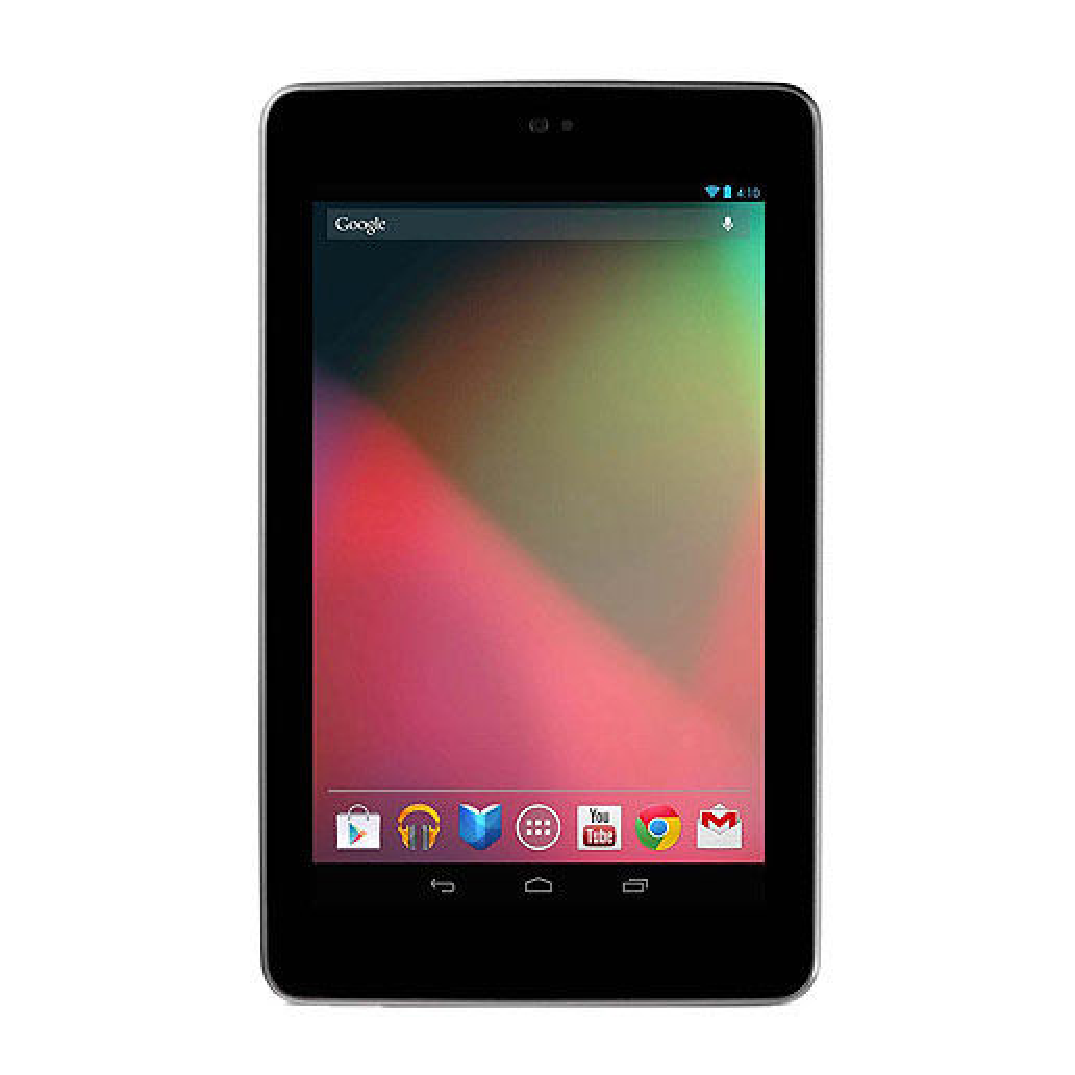
\includegraphics[width=.5\linewidth]{images/nexus7.eps}
  \end{center}
  \caption{Nexus 7}
  \label{fig:nexus7}
\end{figure}

\subsection{被験者}\label{ux88abux9a13ux8005}

被験者は大学生及び大学院生の計n名(男性x名, 女性y名,
平均zz歳)である(表\ref{table:tester})。
いずれの被験者も、情報技術に日頃から触れている。

\begin{longtable}[c]{@{}lrr@{}}
\caption{被験者属性 \label{table:tester}}\tabularnewline
\toprule
被験者ID & 性別 & 年齢\tabularnewline
\midrule
\endfirsthead
\toprule
被験者ID & 性別 & 年齢\tabularnewline
\midrule
\endhead
A & 男 & 26\tabularnewline
B & 男 & 23\tabularnewline
C & 男 & 19\tabularnewline
\bottomrule
\end{longtable}

\subsection{実験タスク}\label{ux5b9fux9a13ux30bfux30b9ux30af}

タスク(課題)は5問用意した。

アプリケーションはフォアグラウンドの状態で、画面を見てもらっている状態でタスクを実行してもらった。

タスク達成時間は、アプリケーションがプログラムからの指示を受け取った時間を開始時間、
人が実行結果を返した時間を終了時間とし、アプリケーションに組み込んだ計測プログラムによって計測した。

タスクの教示方法 条件1
今から実行するプログラムは、コンピュータと人間を同じリソースとして扱えるプログラミング環境で実行されています。
このデバイスに、プログラムからの指示が来るので、それに対して、自分が正しいと思う値を返してください。

\subsection{実験手順}\label{ux5b9fux9a13ux624bux9806}

実験は、2014年12月25日に、慶應義塾大学SFCのデルタS112にて被験者1名ずつで行った(画像)。
被験者には実験用デバイスを手渡し、デバイスに表示される指示に対して、入力を行ってもらうタスク5問を行った。

実験終了後、実行時間や観察内容を元に、インタビューを行った。

\subsection{被験者インタビュー}\label{ux88abux9a13ux8005ux30a4ux30f3ux30bfux30d3ux30e5ux30fc}

実験後、被験者に対して半構造的インタビューを行った。
質問事項を図\ref{table:interview}に示す。

\begin{longtable}[c]{@{}lc@{}}
\caption{インタビュー内容 \label{table:interview}}\tabularnewline
\toprule
& 質問内容\tabularnewline
\midrule
\endfirsthead
\toprule
& 質問内容\tabularnewline
\midrule
\endhead
問1 &
コンピュータと同じ、処理を実行する立場と言われた時、どう思いますか\tabularnewline
問2 &
自分や他人の感性判断をプログラムに組み込むことについて、どう思いますか\tabularnewline
問3 & 返り値のフォーマット指定は 必要でしたか? \tabularnewline
& 考えの幅が狭まるといったことはありますか? \tabularnewline
& 扱いづらいものはありましたか?\tabularnewline
問4 &
好きなキャラや俳優などからの指示のように見えるインタフェースだった場合、\tabularnewline
& 動きに変化があると思いますか?\tabularnewline
問5 &
命令元の人によって、指示に従うかどうかは変わりますか?\tabularnewline
\bottomrule
\end{longtable}

\subsection{実験結果}\label{ux5b9fux9a13ux7d50ux679c}

\subsubsection{反応速度}\label{ux53cdux5fdcux901fux5ea6}

\subsubsection{インタビュー}\label{ux30a4ux30f3ux30bfux30d3ux30e5ux30fc}

\section{性能評価実験}\label{ux6027ux80fdux8a55ux4fa1ux5b9fux9a13}

\subsection{実験趣旨}\label{ux5b9fux9a13ux8da3ux65e8-1}

\ref{sec:user-evaluation}節の実験によって、人間による処理の実行速度を計測した。
本節では、システムの通信部分における速度の計測を行う。
現在実装済みのSocket.IO AdapterとPushNotification
Adapterの二種類の方法について、実験を行う。

\subsection{実験装置}\label{ux5b9fux9a13ux88c5ux7f6e-1}

プログラムを実行する装置には、MacBook Proを用いた。
通信するサーバはHeroku上で運用する。

\subsection{実験内容}\label{ux5b9fux9a13ux5185ux5bb9}

\subsection{実験結果}\label{ux5b9fux9a13ux7d50ux679c-1}

\subsection{考察}\label{ux8003ux5bdf}

\section{まとめ}\label{ux307eux3068ux3081}

本章では、システム利用時における実行速度に関しての実験を行った。
結果として、

\chapter{応用例}\label{chap:application}

本章では、Babascriptプログラミング環境によって実現可能と考えられる応用例について述べる。

\newpage

\section{仕事のプログラム化}\label{ux4ed5ux4e8bux306eux30d7ux30edux30b0ux30e9ux30e0ux5316}

第\ref{chap:background}章でも述べた通り、人間の仕事はマニュアル等によって記述されていることが多い。
マニュアルはどのように行動すべきかが構造的に記述された手順書であり、
「Aという条件の時にはBの処理を実行する」といったことが文章として記述されている。
そのため、これらの手順をソースコードに変換し、プログラムとして実行することは可能と考える。

プログラムとして実行することで、仕事における様々な「状態」をコンピュータに管理させることができる。
この「状態」とは、例えば、進行度が挙げられる。
今までは働いている人間の記憶や知識に依存していた部分をコンピュータに管理させることで、
可能な限りの条件判断を人間が行う処理から外すことが出来る。
コンピュータの判断の元、人間に行動指示が出され、仕事を進行させていくことが可能である。
これにより、個人の経験や知識への依存を減らすことが出来る。
個人への依存は人の代替や引き継ぎを困難にするため、コンピュータによる支援を積極的に行うことで
回避すべきである。

また、プログラム経由での情報のやりとりが増えるため、詳細な実行ログや実行状況をデータとして取得することができる。
これはつまり、仕事の実行量の計測が可能ということである。
作業者がどのように働いていて、どのくらい時間がかかっているのかという情報は、作業者の行動改善に役立つ。
データを元に状況の可視化なども可能である。

プログラムを介することで、人間同士がコミュニケーションを取ることなく、協調して仕事を進めていくことが出来る。
通常、仕事で複数の人が関係してくる場合、当事者同士での相談等、コミュニケーションコストがかかってしまう。
適切に行なわれない場合、遅延等の問題が発生する。
意思決定をコンピュータに委ね、人間による意思決定が必要な場面においては人間に意思判断をさせることで、
コミュニケーションコストを最低限にしつつ複数人による仕事の実行が可能となると考えられる。

\section{人の力を利用した実世界プログラミング}\label{ux4ebaux306eux529bux3092ux5229ux7528ux3057ux305fux5b9fux4e16ux754cux30d7ux30edux30b0ux30e9ux30dfux30f3ux30b0}

人間をセンサーやアクチュエータとして利用することで、人間を使って実世界から情報を得たり、操作することができる。
人間は優秀な入出力装置であり、コンピュータだけでは現在は実現が困難な処理でも実行できるケースがある。
例えば、現在のセンサー技術では、その場の雰囲気の数値化や文字列化といったコンテキストを伴うようなセンシングは困難である。
人間であれば、コンテキストを伴うようなセンシングでも柔軟に解釈し、情報を得ることが出来る。
また、現在のアクチュエータでは、簡単な動作を実行することは容易であるが、複雑な動作となると決められた動きを実行する等限定される。
人間であれば、多少あいまいな指示でも複雑な動作を実現できる。

もちろん、人間が不得意なことやコストを十分に考慮する必要がある。
例えば、正確な温度等の情報を取得するようなことは機械のセンサーを利用するべきである。
人間は知能によって処理が必要となるような情報取得のほうが得意である。
また、定期的に何かを動かしたりすることは、機械のアクチュエータがするべきである。
繰り返し処理や単純な処理は計算機のほうが得意である。

人間とセンサーやアクチュエータを状況に応じて使い分けるという手法も考えられる。
例えば、部屋Aにはセンサーが存在するが、部屋Bにはセンサーが存在しないとして、
部屋Aでプログラムが実行された場合は機械のセンサーを、部屋Bで実行された場合は人間によって
情報の取得を行うというプログラムが実現可能である。

\section{実世界環境の構成管理とテスト}\label{ux5b9fux4e16ux754cux74b0ux5883ux306eux69cbux6210ux7ba1ux7406ux3068ux30c6ux30b9ux30c8}

実世界環境は今後プログラムと密結合していく。
ユビキタスコンピューティング等の実現によって、実世界環境にコンピュータが多く存在し、
プログラムによって制御される空間が実現する。
空間とプログラムは密に結合し、両者を分けて考える事は難しくなると考えられる。
このような実世界環境においても、構成管理やテストをする仕組みが求められる。
つまり、その空間を構成するプログラムとモノであれば、同じようにコードとして記述して構成管理をする必要がある。
しかし、従来の枠組みでは、プログラムの部分のみの構成管理やテストしかできない。
そこでBabascript環境を使うことで、実世界とプログラムの双方を対象とすることができる。
プログラム部分はコンピュータに、実世界の部分に関しては人間によって構成管理を実行したり、テストを行う。

この考えは、サーバやインフラの構成をコードとして記述し、管理するInfrastructure
as Codeという概念を基礎にしている。
従来では、サーバのセットアップは手順書などを元に手動で行っていたが、これをコードとして記述し実行させるというものである。
サーバやインフラの構成をコードで記述しておけば、様々なイベントを元に自動実行が可能であったり、バージョン管理が容易になるため、
新しい構成の構築に失敗しても、すぐに前のバージョンに戻してセットアップが行える。
サーバの構成をテストする仕組みと組み合わせることによって、サーバやインフラさえも、継続的インテグレーションに組み込むことができる。
このように、手順をコードで記述することによって、自動化やテストが可能になるなど有用であることが多い。

空間を制御するプログラムと、そのプログラムが実行されるコンピュータや制御する対象等を含んだ実世界の構成管理と
テストが実現することによって、様々なメリットをユーザは享受出来ると考えられる。
空間の構成がプログラム化されることによって、その空間においてどのような仕組みが動いているのかを形式知として残すことができる。
例えば、増井研究室があるデルタS112という空間では、様々なプログラムが動いており、そのプログラムが動くコンピュータや
制御する対象も様々であるが、その情報は暗黙知に近い状態であると言える。
もし、引っ越しをしたりする場合、実行されなくなってしまうプログラム等も存在すると考えられる。
コンピュータを買い替えたりした場合も同様である。
これらの情報を形式知化し、バージョン管理していくことが出来れば、非常に有用であると言える。

\section{まとめ}\label{ux307eux3068ux3081}

本章では、本提案によって実現が可能と考える応用例について述べた。
人間を利用できることで、今までは実現が困難であったような処理であっても、実現は可能である。

\chapter{考察}\label{chap:discussion}

本章では、Babascriptプログラミング環境における諸問題や
可能性について述べる。

\newpage

\section{ユーザインタビュー}\label{ux30e6ux30fcux30b6ux30a4ux30f3ux30bfux30d3ux30e5ux30fc}

システムの改善や利用者側の心理の確認のため、 7名の被験者(男性7名,
平均23歳)に試用してもらった上でインタビューを行った。
今回のユーザインタビューでは、現状において一番改善点が多いと思われたBabascript
Agentに その議論を絞り、インタビューを行った。

インタビューの内容は表\ref{table:interview}の通りである。

\subsection{プログラムからの指示について}\label{ux30d7ux30edux30b0ux30e9ux30e0ux304bux3089ux306eux6307ux793aux306bux3064ux3044ux3066}

プログラムからの指示を受けるという、コンピュータと人間がまったく同じ立場になるということに関して、
拒否感を覚える人がいるのではないかという仮説を確認するために質問をした。

結果として、被験者全員が特に拒否感を覚えることはないと答えた。
被験者の中には具体的に、プログラムから指示を受けているという印象を受けなかったため、という意見を述べる者もいた。
プログラムからの指示であるという
インタフェースをより洗練させることで、プログラムから指示を受けているという印象を薄めていくことによって、
一般の人にも受け入れてもらえるようにすることは可能と考えられる。

\subsection{自分や他人をプログラムに組み込むことについて}\label{sec:programming-you-and-i}

自分や他人をプログラムに組み込んでみたいと思うのかについて、調査した。
被験者は全員、普段からプログラムを書いている。
そこで、自分や他人を組み込んだプログラムについて、どのようなプログラムがありうるか、
どんなことがポイントになるかについて聞いた。

多くの被験者が、人間を含んだプログラミングは計算機のみを対象としたプログラミングよりも難しくなるのではないかと答えた。
実行する人間によって返ってくる値が異なることが考えられ、想定する値が得られなかった場合の
処理をどうするかについて考える必要がある。

また、被験者の多くは、人間をプログラムに組み込むことには特に抵抗はなく、
様々な処理が楽になる可能性があるならば、使うことが考えられるとの意見を得た。
センサーだけでは得られないデータや、感性による判断を用いたプログラムは有用となる可能性が高いと
答えた被験者も複数存在する。

\subsection{返り値の型について}\label{ux8fd4ux308aux5024ux306eux578bux306bux3064ux3044ux3066}

返り値の型指定について、どう感じたかを質問した。
設計段階より、返り値の型を指定してユーザに提示することで、ユーザは入力しやすくなるのではないかと仮説を立てた。
この仮説について、インタビュー調査において、その検証を行った。
多くの被験者から、型指定によって入力しやすくなったと感じるという意見を得ることができた。
不必要との意見はなく、ユーザの入力の補助になっていると考えられる。

Boolean型とList型は入力がしやすいという意見を多くの被験者から得ることができた。
一方、StringやInt型は、前述の2つの型に比べて入力のコストが高い。
Boolean型やList型に比べて、扱いにくいとの意見を得た。
特に、String型は入力内容の自由度が高いため、入力する値に迷いが生じることが多発しそう、との意見を得た。

\subsection{Babascript Agent
について}\label{babascript-agent-ux306bux3064ux3044ux3066}

\subsubsection{キャラクター性の付与}\label{ux30adux30e3ux30e9ux30afux30bfux30fcux6027ux306eux4ed8ux4e0e}

Babascript Agent
の現在のインタフェースはただ指示を表示し、処理結果を入力させるためだけの機能に絞られている。
このBabascript Agent
に何かしらのキャラクター性をもたせた時、ユーザの挙動がどう変わるかについて、
今後の実装指針とするために聞いた。

好きなキャラクターや俳優など、自分が好意を抱くような対象のキャラクターを持ったインタフェースが提示された場合、
ユーザの意思はどう変わるのかについて聞いた。
半数程度のユーザから、挙動は変化し、比較的指示を聞くようになると思うとの意見を得た。
しかし、この変化を良くないバイアスと評価する人物も存在しており、
単純に良い結果だけを生み出すとは言いにくいと考えられる。

別の意見として、むしろ人間とのコミュニケーションのような形で指示が提示されると良いという意見を得た。
つまり、Siri\footnote{https://www.apple.com/jp/ios/siri/}のような対人型の質問応答システムのような
インタフェースや、チャットのようなインタフェースであれば、プログラムからの指示といった印象が薄れやすいと思われる。

\subsubsection{命令元の提示}\label{ux547dux4ee4ux5143ux306eux63d0ux793a}

Babascript Agent
の現在のインタフェースでは、誰が指示を送っているのかというのがわからない。
命令実行元がどのような立場の人間ならば、ワーカーとして指示に従うか、ということを聞いた。

まず、多くの被験者が身近な人間ならば指示に従うと答えた。
身近な人とは、ここでは家族や自分自身などを示す。
また、上司などの仕事の関係上、上位の立場の人間からの指示であれば、従うと答えた。
これは、第\ref{chap:application}章で述べた「仕事のプログラム化」のような事例において
うまく動作する可能性が高いことを示していると考えられる。
知らない人からの指示に対しては、多くの被験者が従わないと答えた。

指示内容や状況によるという意見もある。
暇なときであれば、指示に応じて行動してしまうかもしれないと述べている。
しかし、この場合、自分にかかる負担に応じて指示に従うかどうかが変わる可能性が高いとも述べている。
自分に負担がほぼかからないような指示であれば、従うことが多いが、
何か大きく行動しなくてはならないという場合や、入力コストが大きすぎる場合は指示を無視する可能性が高いと答えている。

\subsection{その他}\label{ux305dux306eux4ed6}

規定の質問以外にも、インタビューの中で意見を得ることができた。
以下に列挙する。

\begin{itemize}
\itemsep1pt\parskip0pt\parsep0pt
\item
  ただ指示を提示するだけではなく、全体の流れやコンテキストを知りたい
\item
  指示の中でも強調すべきポイントを示したい
\item
  位置情報、音声、写真などを値として返せたら面白い
\item
  比較表現は人によって異なる可能性が高い
\item
  具体的に絞れない指示は理解しづらい
\end{itemize}

\section{処理実行単位としての人}\label{ux51e6ux7406ux5b9fux884cux5358ux4f4dux3068ux3057ux3066ux306eux4eba}

本研究において、人間は処理すべきことを指示され実行する存在、コンピュータやセンサーと同じ処理単位としてみなされる。
ユーザインタビューからコンピュータサイエンスに関する研究を行っている大学生及び大学院生に関しては、
特に抵抗がないということがわかったが、コンピュータサイエンスの知見の少ない一般の人にとっては、
コンピュータと同じ存在ということに心理的な拒否感を覚えるといったことが考えられる。
しかし、処理を指示され実行する立場に徹するということは、指示されたことのみに集中していれば良いということであり、
非常に楽なことでもある。
また、コンピュータに出来ることはコンピュータにやらせ、人間は人間が得意なことや人間にしか出来ないようなことを実行する
ことになるため、ワーカーにとっては作業量が減るなどのメリットも存在する。
指示される立場でいるということは、作業を楽にするための一つのアイデアであるとも言える。

また、指示に積極的に従うことによって、今までは実現出来なかった処理が実現したり、全体的な処理の正確性が向上するとすれば
それはワーカー側にとってもメリットであると言える。

\section{プログラム化のメリット}\label{ux30d7ux30edux30b0ux30e9ux30e0ux5316ux306eux30e1ux30eaux30c3ux30c8}

Babascriptプログラミング環境によって様々な処理をプログラム化した際に得られるメリットについて考察する。

まず、プログラムとして記述しておくことによって、コンピュータと一緒に処理を実行していくことができる。
例えば、普通の計算は明らかにコンピュータのほうが得意だ。
人間のインプット等を元にしてコンピュータに計算させれば、高速かつ正確な結果を得られ、人間も計算しなくて良い。
記憶しておくことも、コンピュータのほうが得意だ。
仕事や実世界の状態をコンピュータで管理することによって、時間が経ったりしても正確に情報を引き出すことが出来る。
一方で、あいまいな出来事の処理や感性的な判断を求められる場面、実世界を対象とした処理などは
人間のほうが得意な場面が多い。
人間と計算機やセンサ・アクチュエータを処理に応じて使い分けることによって、より効率的であったり、正確な処理が実現する。

プログラムとして記述することで、様々な情報を取得が容易になる。
Aという処理にかかった時間は、少し前のプログラムの場合は1分であったが、改善することで30秒にすることができた、
というようなことは、解析プログラムを導入することですぐにわかるだろう。
AさんとBさんが同じ処理を実行した場合の実行時間の差などもデータとして取得することが容易となる。
改善の結果が悪ければすぐに元のプログラムに戻す、といったことも、バージョン管理が一般的に行なわれている
プログラムだからこそ、実行しやすい。

また、複数の人間をオーケストレーションし、効率的に動かすといったことも可能になる。
マニュアルなどでは、基本的に一人の人間を対象としている。
しかし、プログラムで記述し、各自に指示を送るようにすれば、複数の人間の指揮も容易であると考えられる。

\section{型指定}\label{ux578bux6307ux5b9a}

Babascriptプログラミング環境においては、人間への指示に返り値の型を指定することができる。
型はBoolean、String、Number、Selectの4種類が存在し、ユーザにはその型に合ったインタフェースが提示される。

型ごとに入力コストが異なるため、指示の実行終了までの時間が変化すると考えられる。
例えば、String型を指定した場合、文字を入力しなくてはならない。
入力する文字を考える時間や文字入力のスピード、文字入力システムの性能等にも左右される。
一方、Boolean型を指定した場合、2択から選んで決定するだけである。
String型とBoolean型では入力コストに差が存在し、他の2つの型においても同様のことが言える。
可能な限り早く値を返して欲しい場合などは、Boolean型を指定することが望ましい。

型を指定されることによって、ユーザ側も入力すべき値がはっきりとし、迷うことがなかったという意見があった。
一方で、String型の場合、指示内容にもよるが入力の自由度が高くなりがちという問題がある。
String型においては、どんな値を入力すれば良いか迷ったり、わからなかったという意見もあった。
これは、どんな値を入力すべきかという例示をすることによって、ある程度解決可能な問題だと考えられる。

\section{処理の実行遅延と実行保証}\label{ux51e6ux7406ux306eux5b9fux884cux9045ux5ef6ux3068ux5b9fux884cux4fddux8a3c}

Babascriptを用いて人に指示を送っても、指示を受け取った人がその場ですぐに処理を実行するとは限らず、
遅延して実行される可能性がある。
指示を受け取るデバイスを見ていないという場合や、指示を受け取っても状況的にすぐに実行できないという場合があると
考えられ、その場合はすぐに指示に対して実行結果を返すことが出来ない。
Babascriptでは、こういった状況に対応するため、非同期実行を前提とした設計にしている。
そのため、人間による処理の実行中はコンピュータ側に他の処理を実行させておくといったことも可能だが、
人間による処理はほぼ確実に全体の処理を遅延させると考えられる。

また、指示を無視するといったことが起きる可能性があり、実行を完全に保証することができない。
上司からの命令などのように、労働上のある程度の強制力がある場合や、
自分自身への指示、家族からの指示などの場合は、無視の可能性は低くなるが、
強制力がない場合は、指示を無視するといったことが起こりうる。
こういった状況においては、何かしらのインセンティブをワーカーに与えることによって実行保障性を確保することが
できると考えられる。

\section{エラーへの対応}\label{ux30a8ux30e9ux30fcux3078ux306eux5bfeux5fdc}

Babascriptからの指示を受け取った時、その指示が想定している状況と、現実の状況が大きく乖離している可能性がある。
場所や時間に依存するような指示の場合等に発生することが予想される。
指示を受け取った時点や場所においては、指定された型では適切な値を返せないといったことが考えられる。
また、無理やり値を返そうとした結果、本来返されるべき値をは異なる値が処理結果として入力されてしまう可能性も存在する。

Babascript
Agentには、実行出来なかった際などに利用するエラー入力用のインタフェースが存在する。
エラーが起きた際、この機能を適切に利用することでプログラム側に通知が可能だ。
現状の実装では、エラーの内容を文字列として入力するか、デフォルトで指定可能な3つの選択肢から選ぶしかない。
エラーの内容を文字列として表現することは難しく、実際に起きたこととは異なるエラーが報告されてしまう可能性もある。
また、ワーカーへの負担も大きくなる。

また、エラーでプログラムが終了した場合、途中から実行しなおすといったことが現状では出来ない。
実世界におけるタスクの多くは、途中で間違っても、その間違いがタスク継続が困難なものでない限り、途中からやり直すといったことが可能だ。
Babascriptで実現するプログラムにおいても、途中からやり直すという機構が求められる。
Turkit\cite{turkit}におけるcrash-and-rerun
programmingの概念のように、途中経過を保存しておくことで、
プログラムの途中から実行し直すという仕組みが実現可能であると考える。
また、途中経過保存によって、どんなタスクがエラーを起こしやすいのかといったことも保存することができ、
ワークフロー改善にも役立つと考えられる。

\section{処理の先送り}\label{ux51e6ux7406ux306eux5148ux9001ux308a}

プログラムから指示を受け取った時、今でなくても後でなら処理できるという状況が存在する。
しかし、そのまま指示を放置していては、タイムアウト処理等によって指示が撤回されてしまったり、
他の処理が遅延してしまう可能性が高い。
処理の先送りをプログラムに通知しておき、またあとで指示を通知し直すなどの仕組みを用意する必要がある。

これは、Babascirpt
Agent側にも非同期的に指示を通知するインタフェースが必要となる、ということである。
現状では、Babascript Agentは完全に同期的な挙動をする。
先送りした指示や現時点でキューに溜まっている指示などをリスト型のインタフェースで表示しておき、
実行する処理を選べるような設計をすることで、Babascript
Agent側で処理の先送りを実現可能である。

\section{割り込み処理}\label{ux5272ux308aux8fbcux307fux51e6ux7406}

コンピュータが多くの割り込み処理を行っているのと同じように、
様々な指示が送られる中で、人間に対しても、指示を割り込みできるような仕組みが求められる。
例えば、現実においても、割り込み処理は多くなされている。
料理をしてる時に、鍋が吹きこぼれそうだったら、他の処理を中断してでも鍋から吹きこぼれないような処理を行う。

このような割り込み処理を、Babascriptでは、人間の指示構文実行時のオプション情報として
特別なフラグを立てることで実現させている。
人間への指示は、Node-Linda上にキュー形式で保存されているが、
この指示のキューを通常タスクと優先タスクで分けて保存している。
優先タスクキューに指示が入ってる場合は、こちらのキューから優先して指示を取得する。

割り込み処理に関しては、Babascript Agent 側の工夫が非常に重要になる。
実世界における割り込み処理の通知は非常にわかりやすい。
鍋が吹きこぼれそうなら、視覚的にわかりやすく通知が行なわれ、
機械がエラーで止まれば、エラー音による通知が行われる。 Babascript
Agentにおいても、割り込み処理が来た際にはわかりやすく通知することが望ましい。
現状では、高度な工夫は実現できていない。
割り込み処理であるということを明示的にし、割り込んだ処理をすぐに行うように
誘導させられるようにインタフェースを再実装する必要がある。

\section{命令の抽象度設計の必要性}\label{ux547dux4ee4ux306eux62bdux8c61ux5ea6ux8a2dux8a08ux306eux5fc5ux8981ux6027}

Babascriptでは、人への指示構文の記述には制限がない。
そのため、命令の抽象度はプログラマの指示記述能力に依存する。
抽象度が高すぎる指示内容にしてしまうと、ワーカーにとって実行内容が理解しづらくなってしまう。
結果として、想定外の処理が実行されたり、意図しない処理結果を返される可能性が存在する。
人間は柔軟な解釈が可能なため、ある程度は補正可能だと考えられるが、補正が不可能なほど抽象的な
指示内容の場合、問題が発生する。

具体的過ぎる命令は、全体の処理内容にもよるが、プログラム自体が冗長となり得る。
プログラムとワーカーの間のやりとりが増え、通信や待機時間、入力時間などによって処理全体が遅延すると考えられる。
これはワーカーにとっても大きな負担となる。
指示ごとに異なると考えられるが、命令文は適切な抽象度に設計しなくてはならない。

\section{異なる種類の指示の複数同時実行}\label{ux7570ux306aux308bux7a2eux985eux306eux6307ux793aux306eux8907ux6570ux540cux6642ux5b9fux884c}

複数のプログラムから同時に一人の人間に複数の関係のない指示が実行される可能性がある。
例えば、料理プログラムと掃除プログラムが同時に実行された場合、
鍋で何かを煮ている途中に、「洗剤を投入する」といった指示がなされるといったことが考えられる。

現実世界で同じようなことが起きても、人間は指示を分類し、別スレッドで動作させることで問題を回避する。
Babascript Agent
Webアプリケーションプロトタイプ2では、指示を並列に表示させ、
人間側が自分で記憶を元に分類しておくことでこの問題を部分的に解決している。
しかし、類似した指示が来た場合、混同してしまう可能性がある。
どのプログラムからの指示なのかを区別し、
分類し提示するインタフェースを実装することで解決可能と考えられる。

\section{Babascript
Agentへのキャラクター性の付与}\label{babascript-agentux3078ux306eux30adux30e3ux30e9ux30afux30bfux30fcux6027ux306eux4ed8ux4e0e}

Babascript Agentは、一種のソフトウェアエージェントである。 Babascript
Agentを用いた、人とプログラムのコミュニケーションは
ヒューマンエージェントインタラクションであると言える。
ヒューマンエージェントインタラクションとは、
人間とソフトウェアエージェントやロボット間のインタラクション
設計に関する研究分野である。
ヒューマンエージェントインタラクション研究の分野においては、ソフトウェアエージェントやロボットに対して
擬人化手法を適応させることによって、エージェントをより人間らしく見せたり、コミュニケーションを取りやすく
するといった研究がなされている。

擬人化エージェントがもたらす効果については、村上らによる研究\cite{murakami}では、エージェントに人間関係を適応させた実験を行っている。
村上らの実験では、研究室の教官と学生の関係を利用し、教授の顔を模したキャラクターと関係のないキャラクター、両者からの
依頼に対して学生の行動が変化するかどうかを観察した。
実験の結果、教官キャラクターのほうがより依頼を受理されやすいという結果がわかった。
この実験結果から、エージェントに人間関係、特に上司などを模したキャラクターをユーザに提示することである程度、
依頼に対してポジティブにとらえてもらうことが可能だと考えられる。

上記の実験結果は、Babascript Agentにも応用可能である。 Babascript
Agentにキャラクター性を持たせ、そのキャラクターとコミュニケーションを取っているかのように見せる
インタフェースを開発すれば、指示が受理されやすくなる可能性が存在する。
また、キャラクター性の付与によって、プログラムからの指示であるという印象が薄れ、
指示に対する拒否感も薄れるといったことが考えられる。

\section{今後の展望}\label{ux4ecaux5f8cux306eux5c55ux671b}

今後は、本章で述べた問題点についての改善を主に行う。
割り込み処理や処理の先送りは特にBabascript Agent側の改良が必要である。
エラー処理に関する問題も、非常に興味深く、利便性を上げるために解決が必須である。
また、Babascript
Agentへのキャラクター性付与による人間の心理面の変化など、実験の上、その効果を検証したい。

\chapter{関連研究}\label{chap:related}

\section{HumanComputation /
Crowdsourcing}\label{humancomputation-crowdsourcing}

コンピュータの計算能力だけでは解決できない問題を、人間の処理能力を計算資源として利用することによって解決する手法は、
ヒューマンコンピュテーション\cite{humancomputation}と呼ばれ、様々な研究が行なわれている。

\paragraph{reCAPTCHA}\label{recaptcha}

\mbox{}

コンピュータの文字認識能力では処理しきれない文字の認識を人間に実行させるreCAPTCHA\cite{recaptcha}は、
人間かコンピュータかを判別するために文字認識をさせるCAPTCHA\cite{captcha}を応用したものだ。
人間かコンピュータかの判別を行いつつ、未認識の文字の認識をすることができる。
reCAPTCHAを解く人間側にとっては、人間であることを証明しているだけのつもりが、実は文字認識を手伝っている。

\begin{figure}[htbp]
  \begin{center}
  \includegraphics[width=.5\linewidth,bb=0 0 476 316]{images/recaptcha.png}
  \end{center}
  \caption{人間がコンピュータの代わりに文字認識をするシステム reCAPTCHA}
  \label{fig:recaptcha}
\end{figure}

\paragraph{Duolingo}\label{duolingo}

\mbox{}

Duolingo\cite{duolingo}は、ユーザの言語学習における翻訳作業を利用して、ウェブサイトや文書の翻訳を行うアプリケーションだ。
言語学習自体もゲーミフィケーションを活用したものとなっており、翻訳作業しているということは隠蔽された形で語学学習できる。
言語翻訳のための計算資源として人間を利用した事例である。

\paragraph{Vizwiz}\label{vizwiz}

\mbox{}

人間を物体認識エンジンとして利用することのできるVizwiz\cite{vizwiz}というアプリケーションも存在する。
認識したい物体をカメラで撮影し、質問内容などを録音して送ると、インターネットを介して結果を得ることが出来る。
計算機だけでも特定可能な物体に関しては、人力エンジンを介さずに処理することも可能となっている。

\paragraph{Soylent}\label{soylent}

\mbox{}

Soylent\cite{soylent}は、文章の校正をインターネットを介した人間の力を利用して行うソフトウェアだ。
文章を意味が通じる状態を維持して短くしたり、文法的に正しくても意味の通じない文章を意味が通じるようにする作業は、人間のほうが得意である。

\paragraph{CrowdDB}\label{crowddb}

\mbox{}

計算機だけでは処理が困難なクエリに対して、人間を用いることで返答可能にする仕組みとして、
CrowdDB\cite{crowddb}が提案されている。
CrowdSQLという、SQLを拡張したものが記述言語として使われる。

\section{CrowdSourcing}\label{crowdsourcing}

インターネットを介して不特定多数の人間に仕事を依頼する仕組みはクラウドソーシングと呼ばれ、近年注目を浴びている。
クラウドソーシングとは、業務の一部を外部に委託することを示すアウトソーシングという言葉を改変した造語である\cite{riseofcrowdsourcing}。
インターネットを介した不特定多数の人間たち(crowd)に仕事をアウトソースすることから、crowdsourcingと呼ぶ。
非常に安価で、かつ、必要な人員をすぐに確保して仕事依頼が可能なことから、多くの利用例が生まれている。
近年では、Amazon Mechanical
Turk\cite{amt}(以降MTurk)等のクラウドソーシングプラットフォームが登場してきたことによって
多くの利用例が生まれている。
その中でも、本研究と類似している研究について、述べる。

\paragraph{Turkit}\label{turkit}

\mbox{}

Littleらは、このMTurkをプログラムから簡単に利用するためのツールキットであるTurkit\cite{turkit}を提案している。
Turkitでは、通常のプログラミング記法と同じような記法でタスクをクラウドソーシングすることができる\ref{fig:turkit}。
また、クラウドソーシングによる処理結果の保存をしておくことで、その後の処理でプログラム実行に失敗しても
再度クラウドソーシングに処理依頼をするのではなく、保存済みの結果を元にプログラムを再度実行できるような仕組み
であるthe crash-and-return プログラミングモデルを提唱している。
可能な限り従来のプログラミング記法を崩さずに人力処理を組み込むことを目的としており、本研究と類似している。
本研究は、クラウドソーシング処理を前提としておらず、特定の個人に対する指示を実現するものである。
Turkitでは特定個人に対する処理依頼を記述することはできない。
また、MTurkに依存しているため、クライアントサイドなどを自由に記述することはできない。

\begin{figure}[htbp]
  \begin{center}
  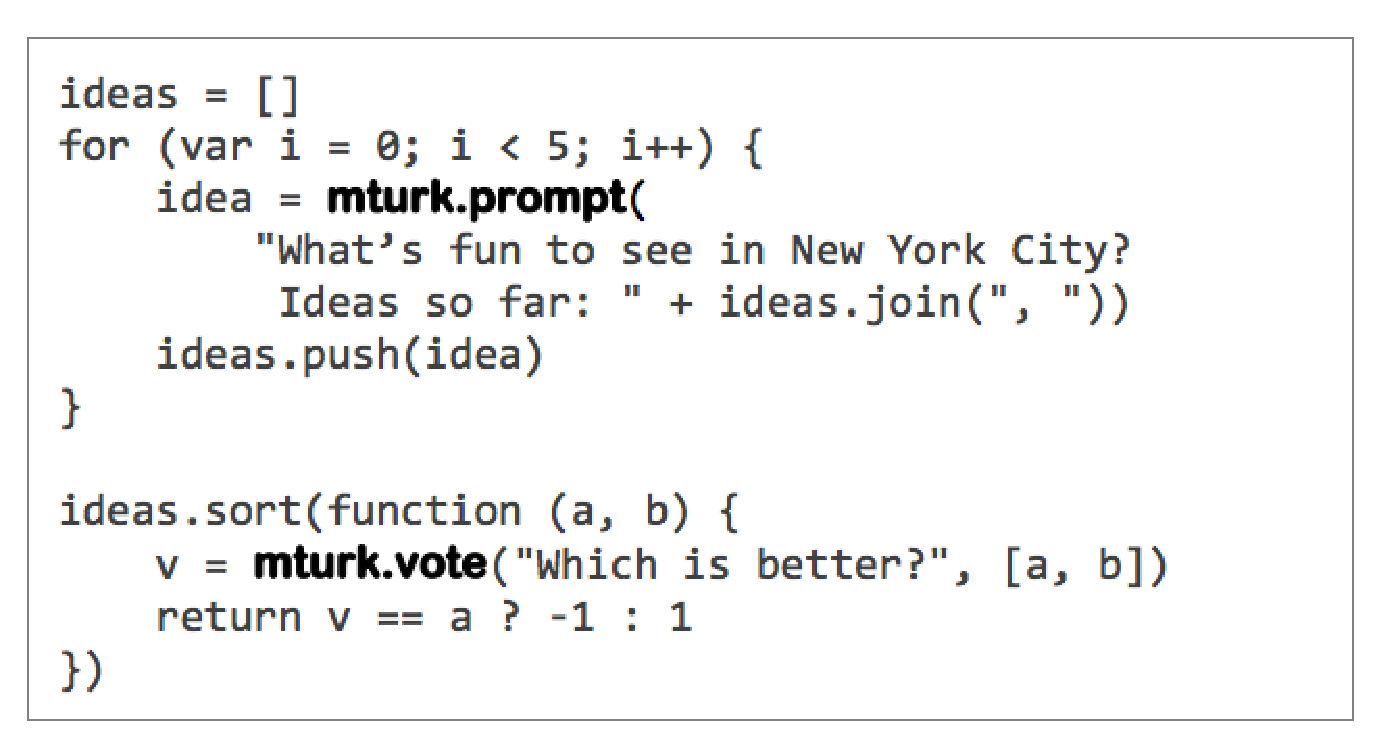
\includegraphics[width=.6\linewidth]{images/turkit.eps}
  \end{center}
  \caption{Turkit}
  \label{fig:turkit}
\end{figure}

\paragraph{Automan}\label{automan}

\mbox{}

Barowyらは、Automanというプログラミング言語Scala上で動作するDomain
Specific Languageを提案した\cite{automan}。
可能な限り通常のプログラミング記法を崩さずにクラウドソーシングを活用した人力処理を組み込むことを目的としており、
クラウドソーシングによる計算とコンピュータによる計算を統合したCrowdProgrammingを提案している。
また、回答の品質管理機能やタスクのスケジューリング、予算の配分等に関する機能を持つ。
本研究における目的は人間と計算機への指示を融合させたプログラミングを実現させることとなっており、類似している。
クラウドソーシング利用を前提としている点や、クライアントアプリケーションを自由に作ることができない点などにおいて
本研究との違いである。

\begin{figure}[htbp]
  \begin{center}
  \includegraphics[width=.6\linewidth,bb=0 0 552 404]{images/automan.png}
  \end{center}
  \caption{Automan}
  \label{fig:automan}
\end{figure}

\paragraph{Cylog}\label{cylog}

\mbox{}

\cite{cylog}

\paragraph{CrowdForge}\label{crowdforge}

\mbox{}

\cite{crowdforge}

\paragraph{Community Based
Crowdsourcing}\label{community-based-crowdsourcing}

\mbox{}

\cite{community-based-crowdsourcing}

\paragraph{Realitime-Captioning}\label{realitime-captioning}

\mbox{}

\cite{realtime-captioning}

クラウドソーシング分野の研究では、インターネットを介して不特定多数の人を計算資源として利用することによって、
コンピュータのみでは実現できなかったような処理や、より大規模な人力処理を実現させている。
本研究では、不特定多数の人ではなく、特定可能な人を対象としたものである。

\section{Social Computing}\label{social-computing}

コンピュータ・ネットワーク上における群衆の様々な行動や叡智をフィードバックデータとして
システムに組み込み活用していくことはソーシャルコンピューティングと呼ばれている。
例えば、群衆による叡智が集められた情報をまとめるためのプラットフォームとしてはWiki\cite{wiki}が存在する。
また、人々が作るwebページのリンク関係から重要度を算出するアルゴリズムとしては、\cite{pagerank}が存在する。
また、群衆の嗜好情報等を蓄積し、個人間の嗜好等の類似度から情報の推薦等を行う手法は協調フィルタリングと呼ばれる\cite{collaborative-filtering}。

次に、特に本研究と関連するソーシャルコンピューティングの事例を紹介する。

\paragraph{The Dog Programming
Language}\label{the-dog-programming-language}

\mbox{}

\cite{dog},

\paragraph{The Jabberwocky Programming
Environmets}\label{the-jabberwocky-programming-environmets}

\mbox{}

\cite{jabberwocky},

\paragraph{Social Machines}\label{social-machines}

\mbox{}

\cite{social-machines},

\paragraph{Human personal apis}\label{human-personal-apis}

\mbox{}

\cite{personal-api},

\section{Human as Sensor}\label{human-as-sensor}

人間をセンサー代わりにしたり、人間が持つスマートフォン等のデバイスのセンサーを利用する手法はHuman
as Sensorと呼ばれる。
ユビキタスコンピューティングなどの研究分野において、こういった手法が多く研究されている。
その事例を以下に紹介する。

\paragraph{PRISM}\label{prism}

\mbox{}

\cite{prism}

\paragraph{Moboq}\label{moboq}

\mbox{}

\cite{moboq}

\paragraph{Medusa}\label{medusa}

\mbox{}

Raらは、medusa\cite{Ra-medusa}という

\paragraph{Mobile Crowdsourcing}\label{mobile-crowdsourcing}

\mbox{}

Huらは、\cite{Hu:mobilecrowdsensing}

\section{Human as Actuator}\label{human-as-actuator}

アクチュエータ技術は進歩しているが、未だに人間のような汎用的に実世界に干渉できる装置はない。
そこで、人間をアクチュエータの代替として利用し動かす、つまり、人間とロボットの協調によって問題を解決しようという研究がある。

\paragraph{HapticTurk}\label{hapticturk}

\mbox{}

Hapticturk\cite{hapticturk}は、人間をモーションプラットフォームのモーターやメカニカル機構の代わりに使うことによって、
モーションプラットフォームの動きを再現するというものだ。
人間への動きの指示はスマートフォンなどを経由して行なわれる。
人間をアクチュエータの代わりに利用するといった点において、本研究と類似している。
本研究では、その用途をアクチュエータに限ったものではない。
また、プログラム上で汎用的に利用可能である。
Hapticturkでは、ゲームにその用途を限定している。

\begin{figure}[htbp]
  \begin{center}
  \includegraphics[width=.6\linewidth,bb=0 0 332 281]{images/hapticturk.png}
  \end{center}
  \caption{Hapticturk}
  \label{fig:hapticturk}
\end{figure}

\paragraph{Sharedo}\label{sharedo}

\mbox{}

加藤らは、ユーザとロボット間のタスクの分業

\cite{sharedo}

\paragraph{グラフィカルデータフローによる調理レシピプログラミング言語の提案}\label{ux30b0ux30e9ux30d5ux30a3ux30abux30ebux30c7ux30fcux30bfux30d5ux30edux30fcux306bux3088ux308bux8abfux7406ux30ecux30b7ux30d4ux30d7ux30edux30b0ux30e9ux30dfux30f3ux30b0ux8a00ux8a9eux306eux63d0ux6848}

\mbox{}

吉川らは調理レシピを記述するためのデータフロープログラミング言語を提案している\cite{recipe-programming}。
料理レシピをグラフィカルなデータフローで記述する。
料理レシピプログラムは、コンピュータではなく人間が実行するためのも
のだ。
本研究のように、人間がプログラムからの指示を実行することを前提としたものとなっている。

\paragraph{Cooky}\label{cooky}

\mbox{}

Sugiuraらは、人間とロボットが協調して調理をするシステムCooky\cite{cooky}を提案している。
料理支援ロボットと人とロボットが共有可能な調理器具やキッチン、調理手順を記述するシステムから成り立っている。
調理手順記述システムでは、人間とロボット双方の処理を分けて記述することができる。
人間とロボットが協調して作業を実行していくモデルは、本研究が目的とするモデルと類似する。
また、人間の作業タイミング時に、人間に作業内容を提示するなど、類似する点は多い。

\begin{figure}[htbp]
  \begin{center}
  \includegraphics[width=.6\linewidth,bb=0 0 633 336]{images/cooky.png}
  \end{center}
  \caption{Cooky}
  \label{fig:cooky}
\end{figure}

\section{ワークフロー系}\label{ux30efux30fcux30afux30d5ux30edux30fcux7cfb}

仕事などにおけるプロセスを文書などによってパターンとして規定し、検証や再利用しやすくするためのものとして
ワークフローというものがある。
このワークフローを構築するための仕組みが複数存在する。

YAWL\cite{yawl}は、ワークフローやビジネス・プロセスを記述するためのワークフロー記述言語だ。
類似のものとしては、XPDL(XML Process Definition
Language)\cite{xpdl}が存在する。
これらのワークフロー記述言語を実行するワークフローエンジンと呼ばれるソフトウェアも多く存在する。
ワークフロー記述言語は、ワークフローを記述するものである。
プログラムによる処理を記述することはできない。

また、X-point\footnote{https://www.atled.jp/xpoint/}や
questetra\footnote{http://www.questetra.com/ja/}といった
ワークフロー記述・実行のためのWebサービスも存在する。

\chapter{結論}\label{chap:conclusion}

本章では、本論文を統括する。

\section{論文の統括と結論}\label{ux8ad6ux6587ux306eux7d71ux62ecux3068ux7d50ux8ad6}

本論文では、人間と計算機の処理を融合させたプログラミング環境の設計と実装を行った。
また、提案したプログラミング環境における人間の応答速度を明らかにした。

プログラムは今後さらにその処理領域を広め、社会と生活、世界を構成する重要な要素となっていく。
また、人間も計算資源としてシステムに組み込まれ、人間と計算機が協働して様々な処理を実現していくと予想される。

既存研究においても人間を計算資源として利用する研究はなされているが、それらの研究では人間の知能を組み込む
レベルの統合しか果たされていない。
人間は知能だけが優秀なのではなく、その身体と知能の両方を利用することで最大限の力を発揮する。
身体操作の指示まで踏み込んだ人間と計算機への指示の融合を実現させたプログラミング環境が必要である。

そこで、自分自身や家族等、身近な人間を計算資源として統合し、普通のプログラミング記法で記述・実行可能な
プログラミング環境について提案した。
この仕組みによって、より簡単に人間をプログラムに組み込んで、実世界におけるタスクを含んだプログラムを
実行することが可能になる。
仕事のプログラム化等、プログラムによって人間の行動をサポートすることができるなど、
有用性のあるプログラミング環境であると言える。

今後は、システムの改良や、考察で述べた点についての改善などを行うことで、
より有用なシステムにしていく。


\begin{acknowledgment}

修士課程の2年間、研究をご指導いただいてきた慶應義塾大学環境情報学部の増井俊之教授に深く感謝致します。
また、本研究の副査としてご意見、ご助言を頂きました徳田教授、田中准教授に感謝致します。

インタラクションデザインプロジェクトに在籍し、メンバーたちと多くの議論をすることができました。
橋本翔さんには、初期の頃よりBabascriptについて多くの議論していただきました。
橋本さんがいなければ、Babascriptが研究として発表されることはなかったと思われます。感謝いたします。
研究・私生活ともに、同期の皆様には様々な面において支えられてきました。
臼杵壮也さん、郡山隼人さん,田中優さんに感謝します。
中園翔さんと桜井雄介さんには、iDPのメンバーとして様々な意見を頂きました。
また、中園さんには本論文の校正も手伝っていただきました。
感謝します。
増井研究室の学部生の皆様にも感謝します。

本研究は、独立行政法人情報処理推進機構 2013年度未踏IT人材発掘・育成事業の支援を受けました。
未踏事業の中でプロジェクトマネージャーとして多くの助言を頂きました大阪大学の石黒浩教授に感謝致します。
未踏事業の同期のメンバーとは、研究を進めていく上で重要となった議論を多く交わすことができました。
また、多くのOBの方々にもアドバイスを頂きました。感謝致します。

修士論文執筆にあたっては、学部時代の先輩にあたる黒井さんと山本伶さんが作ったテンプレートを使用させていただきました。
また、山本伶さんには、本論文の校正を手伝っていただきました。感謝いたします。
片倉弘貴さんには、在学中にプログラミングに関して、Babascriptに関して多くのアドバイスを頂きました。
片倉さんとの議論は本研究に大きな影響を与えています。また、本論文の校正も手伝ってもらいました。感謝します。
秋山博紀さんには、学部生の頃より様々なアドバイスを頂きました。
また、元イオタの民たちには、修士生活で悩んだことの多くを相談させていただき、
的確なアドバイスをいただきました。感謝いたします。

最後に、大学に泊まることが多く、中々家に帰ってこない私の身をいつも心配してくれていた両親と、
実装に関するアドバイスを始め、技術的な話に付き合ってくれた兄に感謝いたします。ありがとうございます。

\end{acknowledgment}
  % 謝辞。要独自コマンド、include先参照のこと

\include{tex/publication}

\include{tex/bibliography}  % 参考文献。要独自コマンド、include先参照のこと
\appendix
\chapter{付録}\label{chap:appendix}

\section{インタビュー調査
被験者属性}\label{ux30a4ux30f3ux30bfux30d3ux30e5ux30fcux8abfux67fb-ux88abux9a13ux8005ux5c5eux6027}

\begin{longtable}[c]{@{}lrr@{}}
\toprule
被験者ID & 性別 & 年齢\tabularnewline
\midrule
\endhead
01 & 男 & 19\tabularnewline
02 & 男 & 23\tabularnewline
03 & 男 & 25\tabularnewline
04 & 男 & 25\tabularnewline
05 & 男 & 26\tabularnewline
06 & 男 & 24\tabularnewline
07 & 男 & 19\tabularnewline
\bottomrule
\end{longtable}
    % 付録

\end{document}
